% generated by Docutils <http://docutils.sourceforge.net/>
\documentclass[a4paper,english]{article}
\usepackage{fixltx2e} % LaTeX patches, \textsubscript
\usepackage{cmap} % fix search and cut-and-paste in PDF
\usepackage[T1]{fontenc}
\usepackage[utf8]{inputenc}
\usepackage{ifthen}
\usepackage{babel}
\usepackage{float} % float configuration
\floatplacement{figure}{H} % place figures here definitely
\usepackage{graphicx}
\usepackage{longtable}
\usepackage{array}
\setlength{\extrarowheight}{2pt}
\newlength{\DUtablewidth} % internal use in tables

%%% Custom LaTeX preamble
% PDF Standard Fonts
\usepackage{mathptmx} % Times
\usepackage[scaled=.90]{helvet}
\usepackage{courier}

%%% User specified packages and stylesheets

%%% Fallback definitions for Docutils-specific commands

% fieldlist environment
\ifthenelse{\isundefined{\DUfieldlist}}{
  \newenvironment{DUfieldlist}%
    {\quote\description}
    {\enddescription\endquote}
}{}

% titlereference role
\providecommand*{\DUroletitlereference}[1]{\textsl{#1}}

% hyperlinks:
\ifthenelse{\isundefined{\hypersetup}}{
  \usepackage[unicode,colorlinks=true,linkcolor=blue,urlcolor=blue]{hyperref}
  \urlstyle{same} % normal text font (alternatives: tt, rm, sf)
}{}

%%% Body
\begin{document}

% Automatically generated reST file from Doconce source
% (http://code.google.com/p/doconce/)


%___________________________________________________________________________

\section*{Doconce Description%
  \phantomsection%
  \addcontentsline{toc}{section}{Doconce Description}%
  \label{doconce-description}%
}
%
\begin{DUfieldlist}
\item[{Author:}]
Hans Petter Langtangen

\item[{Date:}]
Feb 20, 2011

\end{DUfieldlist}

% lines beginning with # are comment lines


%___________________________________________________________________________

\section*{What Is Doconce?%
  \phantomsection%
  \addcontentsline{toc}{section}{What Is Doconce?}%
  \label{id1}%
  \label{what-is-doconce}%
}

Doconce is two things:
%
\begin{quote}
\newcounter{listcnt0}
\begin{list}{\arabic{listcnt0}.}
{
\usecounter{listcnt0}
\setlength{\rightmargin}{\leftmargin}
}

\item Doconce is a very simple and minimally tagged markup language that
look like ordinary ASCII text (much like what you would use in an
email), but the text can be transformed to numerous other formats,
including HTML, Wiki, LaTeX, PDF, reStructuredText (reST), Sphinx,
Epytext, and also plain text (where non-obvious formatting/tags are
removed for clear reading in, e.g., emails). From reStructuredText
you can go to XML, HTML, LaTeX, PDF, OpenOffice, and from the
latter to RTF and MS Word.

\item Doconce is a working strategy for never duplicating information.
Text is written in a single place and then transformed to
a number of different destinations of diverse type (software
source code, manuals, tutorials, books, wikis, memos, emails, etc.).
The Doconce markup language support this working strategy.
The slogan is: ``Write once, include anywhere''.
\end{list}

\end{quote}

A wide range of markup languages exist. For example, reStructuredText and Sphinx
have recently become popular. So why another one?
%
\begin{quote}
%
\begin{itemize}

\item Doconce can convert to plain \emph{untagged} text,
more desirable for computer programs and email.

\item Doconce has less cluttered tagging of text.

\item Doconce has better support for copying in parts of computer code,
say in examples, directly from the source code files.

\item Doconce has stronger support for mathematical typesetting, and
has many features for being integrated with (big) LaTeX projects.

\item Doconce is almost self-explanatory and is a handy starting point
for generating documents in more complicated markup languages, such
as Google Wiki, LaTeX, and Sphinx. A primary application of Doconce
is just to make the initial versions of a Sphinx or Wiki document.

\end{itemize}

\end{quote}

Doconce was particularly written for the following sample applications:
%
\begin{quote}
%
\begin{itemize}

\item Large books written in LaTeX, but where many pieces (computer demos,
projects, examples) can be written in Doconce to appear in other
contexts in other formats, including plain HTML, Sphinx, or MS Word.

\item Software documentation, primarily Python doc strings, which one wants
to appear as plain untagged text for viewing in Pydoc, as reStructuredText
for use with Sphinx, as wiki text when publishing the software at
googlecode.com, and as LaTeX integrated in, e.g., a thesis.

\item Quick memos, which start as plain text in email, then some small
amount of Doconce tagging is added, before the memos can appear as
MS Word documents or in wikis.

\end{itemize}

\end{quote}

Disclaimer: Doconce is a simple tool, largely based on interpreting
and handling text through regular expressions. The possibility for
tweaking the layout is obviously limited since the text can go to
all sorts of sophisticated markup languages. Moreover, because of
limitations of regular expressions, some formatting may face problems
when transformed to other formats.

You can jump to the section \hyperref[the-doconce-software-documentation-strategy]{The Doconce Software Documentation Strategy} to see a recipe for
how to use Doconce, unless you need some more motivation for
the problem which Doconce tries to solve.


%___________________________________________________________________________

\section*{Motivation: Problems with Documenting Software%
  \phantomsection%
  \addcontentsline{toc}{section}{Motivation: Problems with Documenting Software}%
  \label{motivation-problems-with-documenting-software}%
}

\emph{Duplicated Information.} It is common to write some software
documentation in the code (doc strings in Python, doxygen in C++,
javadoc in Java) while similar documentation is often also included in
a LaTeX or HTML manual or tutorial. Although the various types of
documentation may start out to be the same, different physical files
must be used since very different tagging is required for different
output formats. Over time the duplicated information starts to
diverge. Severe problems with such unsynchronized documentation was
one motivation for developing the Doconce concept and tool.

\emph{Tagging Issues in Python Documentation.} A problem with doc
strings in Python is that they benefit greatly from some tagging,
Epytext or reStructuredText, when transformed to HTML or PDF
manuals. However, such tagging looks annoying in Pydoc, which just
shows the pure doc string. For Pydoc we should have more minimal (or
no) tagging (students and newbies are in particular annoyed by any
unfamiliar tagging of ASCII text). On the contrary, manuals or
tutorials in HTML and LaTeX need quite much tagging.

\emph{Solution.} Accurate information is crucial and can only be
maintained in a \emph{single physical} place (file), which must be
converted (filtered) to suitable formats and included in various
documents (HTML/LaTeX manuals/tutorials, Pydoc/Epydoc/HappyDoc
reference manuals).

\emph{A Common Format.} There is no existing format and associated
conversion tools that allow a ``singleton'' documentation file to be
filtered to LaTeX, HTML, XML, PDF, Epydoc, HappyDoc, Pydoc, \emph{and} plain
untagged text. As we are involved with mathematical software, the
LaTeX manuals should have nicely typeset mathematics, while Pydoc,
Epydoc, and HappyDoc must show LaTeX math in verbatim mode.
Unfortunately, Epytext is annoyed by even very simple LaTeX math (also
in verbatim environments). To summarize, we need
%
\begin{quote}
\setcounter{listcnt0}{0}
\begin{list}{\arabic{listcnt0}.}
{
\usecounter{listcnt0}
\setlength{\rightmargin}{\leftmargin}
}

\item A minimally tagged markup language with full support for
for mathematics and verbatim computer code.

\item Filters for producing highly tagged formats (LaTeX, HTML, XML),
medium tagged formats (reStructuredText, Epytext), and plain
text with completely invivisble tagging.

\item Tools for inserting appropriately filtered versions of a ``singleton''
documentation file in other documents (manuals, tutorials, doc strings).
\end{list}

\end{quote}

One answer to these points is the Doconce markup language, its
associated tools, and a \href{http://code.google.com/p/preprocess}{C-style preprocessor tool} or the \href{http://www.makotemplates.org/}{Mako template system}.  Then we can \emph{write once, include
anywhere}!  And what we write is close to plain ASCII text.

But isn't reStructuredText exactly the format that fulfills the needs
above? Yes and no. Yes, because reStructuredText can be filtered to a
lot of the mentioned formats. No, because of the reasons listed
in the section \hyperref[id1]{What Is Doconce?}, but perhaps the strongest feature
of Doconce is that it integrates well with LaTeX: Large LaTeX documents (book)
can be made of many smaller Doconce units, typically describing examples
and computer codes, glued with mathematical pieces written entirely
in LaTeX and with heavy cross-referencing of equations, as is usual
in mathematical texts. All the Doconce units can then be available
also as stand-alone examples in wikis or Sphinx pages and thereby used
in other occasions (including software documentation and teaching material).
This is a promising way of composing future books of units that can
be reused in many contexts and formats, currently being explored by
the Doconce maintainer.

A final warning may be necessary: The Doconce format is a minimalistic
formatting language. It is ideal when you start a new project when you
are uncertain about which format to choose. At some later stage, when
you need quite some sophisticated formatting and layout, you can
perform the final filtering of Doconce into something more appropriate
for future demands. The convenient thing is that the format decision
can be posponed (maybe forever - which is the common experience of the
Doconce developer).


%___________________________________________________________________________

\subsection*{Dependencies%
  \phantomsection%
  \addcontentsline{toc}{subsection}{Dependencies}%
  \label{dependencies}%
}

If you make use of preprocessor directives in the Doconce source,
either \href{http://code.google.com/p/preprocess}{Preprocess} or \href{http://www.makotemplates.org}{Mako} must be installed.  To make LaTeX
documents (without going through the reStructuredText format) you also
need \href{http://code.google.com/p/ptex2tex}{ptex2tex} and some style
files that \texttt{ptex2tex} potentially makes use of.  Going from
reStructuredText to formats such as XML, OpenOffice, HTML, and LaTeX
requires \href{http://docutils.sourceforge.net}{docutils}.  Making Sphinx
documents requires of course \href{http://sphinx.pocoo.org}{Sphinx}.
All of the mentioned potential dependencies are pure Python packages
which are easily installed.


%___________________________________________________________________________

\subsection*{The Doconce Software Documentation Strategy%
  \phantomsection%
  \addcontentsline{toc}{subsection}{The Doconce Software Documentation Strategy}%
  \label{the-doconce-software-documentation-strategy}%
  \label{doconce-strategy}%
}
%
\begin{quote}
%
\begin{itemize}

\item Write software documentation, both tutorials and manuals, in
the Doconce format. Use many files - and never duplicate information!

\item Use \texttt{\#include} statements in source code (especially in doc
strings) and in LaTeX documents for including documentation
files.  These documentation files must be filtered to an
appropriate format by the program \texttt{doconce} before being
included. In a Python context, this means plain text for computer
source code (and Pydoc); Epytext for Epydoc API documentation, or
the Sphinx dialect of reStructuredText for Sphinx API
documentation; LaTeX for LaTeX manuals; and possibly
reStructuredText for XML, Docbook, OpenOffice, RTF, Word.

\item Run the preprocessor \texttt{preprocess} on the files to produce native
files for pure computer code and for various other documents.

\end{itemize}

\end{quote}

Consider an example involving a Python module in a \texttt{basename.p.py} file.
The \texttt{.p.py} extension identifies this as a file that has to be
preprocessed) by the \texttt{preprocess} program.
In a doc string in \texttt{basename.p.py} we do a preprocessor include
in a comment line, say (use triple quotes in the doc string in case
the \texttt{doc1} documentation includes code snippets with doc strings
with the usual triple double quotes):
%
\begin{quote}{\ttfamily \raggedright \noindent
'{}'{}'\\
\#~~~~\#include~"docstrings/doc1.dst.txt\\
'{}'{}'
}
\end{quote}

% Note: we insert an error right above as the right quote is missing.

% Then preprocess skips the statement, otherwise it gives an error

% message about a missing file docstrings/doc1.dst.txt (which we don't

% have, it's just a sample file name). Also note that comment lines

% must not come before a code block for the rst/st/epytext formats to work.

The file \texttt{docstrings/doc1.dst.txt} is a file filtered to a specific format
(typically plain text, reStructedText, or Epytext) from an original
``singleton'' documentation file named \texttt{docstrings/doc1.do.txt}. The \texttt{.dst.txt}
is the extension of a file filtered ready for being included in a doc
string (\texttt{d} for doc, \texttt{st} for string).

For making an Epydoc manual, the \texttt{docstrings/doc1.do.txt} file is
filtered to \texttt{docstrings/doc1.epytext} and renamed to
\texttt{docstrings/doc1.dst.txt}.  Then we run the preprocessor on the
\texttt{basename.p.py} file and create a real Python file
\texttt{basename.py}. Finally, we run Epydoc on this file. Alternatively, and
nowadays preferably, we use Sphinx for API documentation and then the
Doconce \texttt{docstrings/doc1.do.txt} file is filtered to
\texttt{docstrings/doc1.rst} and renamed to \texttt{docstrings/doc1.dst.txt}. A
Sphinx directory must have been made with the right \texttt{index.rst} and
\texttt{conf.py} files. Going to this directory and typing \texttt{make html} makes
the HTML version of the Sphinx API documentation.

The next step is to produce the final pure Python source code. For
this purpose we filter \texttt{docstrings/doc1.do.txt} to plain text format
(\texttt{docstrings/doc1.txt}) and rename to \texttt{docstrings/doc1.dst.txt}. The
preprocessor transforms the \texttt{basename.p.py} file to a standard Python
file \texttt{basename.py}. The doc strings are now in plain text and well
suited for Pydoc or reading by humans. All these steps are automated
by the \texttt{insertdocstr.py} script.  Here are the corresponding Unix
commands:
%
\begin{quote}{\ttfamily \raggedright \noindent
\#~make~Epydoc~API~manual~of~basename~module:\\
cd~docstrings\\
doconce~format~epytext~doc1.do.txt\\
mv~doc1.epytext~doc1.dst.txt\\
cd~..\\
preprocess~basename.p.py~>~basename.py\\
epydoc~basename\\
~\\
\#~make~Sphinx~API~manual~of~basename~module:\\
cd~doc\\
doconce~format~sphinx~doc1.do.txt\\
mv~doc1.rst~doc1.dst.txt\\
cd~..\\
preprocess~basename.p.py~>~basename.py\\
cd~docstrings/sphinx-rootdir~~\#~sphinx~directory~for~API~source\\
make~clean\\
make~html\\
cd~../..\\
~\\
\#~make~ordinary~Python~module~files~with~doc~strings:\\
cd~docstrings\\
doconce~format~plain~doc1.do.txt\\
mv~doc1.txt~doc1.dst.txt\\
cd~..\\
preprocess~basename.p.py~>~basename.py\\
~\\
\#~can~automate~inserting~doc~strings~in~all~.p.py~files:\\
insertdocstr.py~plain~.\\
\#~(runs~through~all~.do.txt~files~and~filters~them~to~plain~format~and\\
\#~renames~to~.dst.txt~extension,~then~the~script~runs~through~all\\
\#~.p.py~files~and~runs~the~preprocessor,~which~includes~the~.dst.txt\\
\#~files)
}
\end{quote}

% some comment lines that do not affect any formatting

% these lines are simply removed


%___________________________________________________________________________

\subsection*{Demos%
  \phantomsection%
  \addcontentsline{toc}{subsection}{Demos}%
  \label{demos}%
}

The current text is generated from a Doconce format stored in the:
%
\begin{quote}{\ttfamily \raggedright \noindent
docs/manual/manual.do.txt
}
\end{quote}

file in the Doconce source code tree. We have made a
\href{https://doconce.googlecode.com/hg/trunk/docs/demos/manual/index.html}{demo web page}
where you can compare the Doconce source with the output in many
different formats: HTML, LaTeX, plain text, etc.

The file \texttt{make.sh} in the same directory as the \texttt{manual.do.txt} file
(the current text) shows how to run \texttt{doconce format} on the
Doconce file to obtain documents in various formats.

Another demo is found in:
%
\begin{quote}{\ttfamily \raggedright \noindent
docs/tutorial/tutorial.do.txt
}
\end{quote}

In the \texttt{tutorial} directory there is also a \texttt{make.sh} file producing a
lot of formats, with a corresponding
\href{https://doconce.googlecode.com/hg/trunk/docs/demos/tutorial/index.html}{web demo}
of the results.

% Example on including another Doconce file:


%___________________________________________________________________________

\section*{From Doconce to Other Formats%
  \phantomsection%
  \addcontentsline{toc}{section}{From Doconce to Other Formats}%
  \label{from-doconce-to-other-formats}%
  \label{doconce2formats}%
}

Transformation of a Doconce document to various other
formats applies the script \texttt{doconce format}:
%
\begin{quote}{\ttfamily \raggedright \noindent
Unix/DOS>~doconce~format~format~mydoc.do.txt
}
\end{quote}

The \texttt{preprocess} program is always used to preprocess the file first,
and options to \texttt{preprocess} can be added after the filename. For example:
%
\begin{quote}{\ttfamily \raggedright \noindent
Unix/DOS>~doconce~format~LaTeX~mydoc.do.txt~-Dextra\_sections
}
\end{quote}

The variable \texttt{FORMAT} is always defined as the current format when
running \texttt{preprocess}. That is, in the last example, \texttt{FORMAT} is
defined as \texttt{LaTeX}. Inside the Doconce document one can then perform
format specific actions through tests like \texttt{\#if FORMAT == "LaTeX"}.

Inline comments in the text are removed from the output by:
%
\begin{quote}{\ttfamily \raggedright \noindent
Unix/DOS>~doconce~format~LaTeX~mydoc.do.txt~remove\_inline\_comments
}
\end{quote}

One can also remove such comments from the original Doconce file
by running a helper script in the \texttt{bin} folder of the Doconce
source code:
%
\begin{quote}{\ttfamily \raggedright \noindent
Unix/DOS>~doconce~remove\_inline\_comments~mydoc.do.txt
}
\end{quote}

This action is convenient when a Doconce document reaches its final form.


%___________________________________________________________________________

\subsection*{HTML%
  \phantomsection%
  \addcontentsline{toc}{subsection}{HTML}%
  \label{html}%
}

Making an HTML version of a Doconce file \texttt{mydoc.do.txt}
is performed by:
%
\begin{quote}{\ttfamily \raggedright \noindent
Unix/DOS>~doconce~format~HTML~mydoc.do.txt
}
\end{quote}

The resulting file \texttt{mydoc.html} can be loaded into any web browser for viewing.


%___________________________________________________________________________

\subsection*{LaTeX%
  \phantomsection%
  \addcontentsline{toc}{subsection}{LaTeX}%
  \label{latex}%
}

Making a LaTeX file \texttt{mydoc.tex} from \texttt{mydoc.do.txt} is done in two steps:
.. Note: putting code blocks inside a list is not successful in many
.. formats - the text may be messed up. A better choice is a paragraph
.. environment, as used here.
%
\begin{description}
\item[{\emph{Step 1.} Filter the doconce text to a pre-LaTeX form \texttt{mydoc.p.tex} for}] \leavevmode 
\texttt{ptex2tex}:
%
\begin{quote}{\ttfamily \raggedright \noindent
Unix/DOS>~doconce~format~LaTeX~mydoc.do.txt
}
\end{quote}

\end{description}

LaTeX-specific commands (``newcommands'') in math formulas and similar
can be placed in files \texttt{newcommands.tex}, \texttt{newcommands\_keep.tex}, or
\texttt{newcommands\_replace.tex} (see the section \hyperref[macros-newcommands]{Macros (Newcommands)}).
If these files are present, they are included in the LaTeX document
so that your commands are defined.

\emph{Step 2.} Run \texttt{ptex2tex} (if you have it) to make a standard LaTeX file:
%
\begin{quote}{\ttfamily \raggedright \noindent
Unix/DOS>~ptex2tex~mydoc
}
\end{quote}

or just perform a plain copy:
%
\begin{quote}{\ttfamily \raggedright \noindent
Unix/DOS>~cp~mydoc.p.tex~mydoc.tex
}
\end{quote}

Doconce generates a \texttt{.p.tex} file with some preprocessor macros.
For example, to enable font Helvetica instead of the standard
Computer Modern font:
%
\begin{quote}{\ttfamily \raggedright \noindent
Unix/DOS>~ptex2tex~-DHELVETICA~mydoc
}
\end{quote}

The title, authors, and date are by default typeset in a non-standard
way to enable a nicer treatment of multiple authors having
institutions in common. The standard LaTeX ``maketitle'' heading
is also available through:
%
\begin{quote}{\ttfamily \raggedright \noindent
Unix/DOS>~ptex2tex~-DTRAD\_LATEX\_HEADING~mydoc
}
\end{quote}

The \texttt{ptex2tex} tool makes it possible to easily switch between many
different fancy formattings of computer or verbatim code in LaTeX
documents. After any \texttt{!bc sys} command in the Doconce source you can
insert verbatim block styles as defined in your \texttt{.ptex2tex.cfg}
file, e.g., \texttt{!bc sys cod} for a code snippet, where \texttt{cod} is set to
a certain environment in \texttt{.ptex2tex.cfg} (e.g., \texttt{CodeIntended}).
There are over 30 styles to choose from.

\emph{Step 3.} Compile \texttt{mydoc.tex}
and create the PDF file:
%
\begin{quote}{\ttfamily \raggedright \noindent
Unix/DOS>~latex~mydoc\\
Unix/DOS>~latex~mydoc\\
Unix/DOS>~makeindex~mydoc~~~\#~if~index\\
Unix/DOS>~bibitem~mydoc~~~~~\#~if~bibliography\\
Unix/DOS>~latex~mydoc\\
Unix/DOS>~dvipdf~mydoc
}
\end{quote}

If one wishes to use the \texttt{Minted\_Python}, \texttt{Minted\_Cpp}, etc., environments
in \texttt{ptex2tex} for typesetting code, the \texttt{minted} LaTeX package is needed.
This package is included by running \texttt{doconce format} with the
\texttt{-DMINTED} option:
%
\begin{quote}{\ttfamily \raggedright \noindent
Unix/DOS>~ptex2tex~-DMINTED~mydoc
}
\end{quote}

In this case, \texttt{latex} must be run with the
\texttt{-shell-escape} option:
%
\begin{quote}{\ttfamily \raggedright \noindent
Unix/DOS>~latex~-shell-escape~mydoc\\
Unix/DOS>~latex~-shell-escape~mydoc\\
Unix/DOS>~makeindex~mydoc~~~\#~if~index\\
Unix/DOS>~bibitem~mydoc~~~~~\#~if~bibliography\\
Unix/DOS>~latex~-shell-escape~mydoc\\
Unix/DOS>~dvipdf~mydoc
}
\end{quote}

The \texttt{-shell-escape} option is required because the \texttt{minted.sty} style
file runs the \texttt{pygments} program to format code, and this program
cannot be run from \texttt{latex} without the \texttt{-shell-escape} option.


%___________________________________________________________________________

\subsection*{Plain ASCII Text%
  \phantomsection%
  \addcontentsline{toc}{subsection}{Plain ASCII Text}%
  \label{plain-ascii-text}%
}

We can go from Doconce ``back to'' plain untagged text suitable for viewing
in terminal windows, inclusion in email text, or for insertion in
computer source code:
%
\begin{quote}{\ttfamily \raggedright \noindent
Unix/DOS>~doconce~format~plain~mydoc.do.txt~~\#~results~in~mydoc.txt
}
\end{quote}


%___________________________________________________________________________

\subsection*{reStructuredText%
  \phantomsection%
  \addcontentsline{toc}{subsection}{reStructuredText}%
  \label{restructuredtext}%
}

Going from Doconce to reStructuredText gives a lot of possibilities to
go to other formats. First we filter the Doconce text to a
reStructuredText file \texttt{mydoc.rst}:
%
\begin{quote}{\ttfamily \raggedright \noindent
Unix/DOS>~doconce~format~rst~mydoc.do.txt
}
\end{quote}

We may now produce various other formats:
%
\begin{quote}{\ttfamily \raggedright \noindent
Unix/DOS>~rst2html.py~~mydoc.rst~>~mydoc.html~\#~HTML\\
Unix/DOS>~rst2latex.py~mydoc.rst~>~mydoc.tex~~\#~LaTeX\\
Unix/DOS>~rst2xml.py~~~mydoc.rst~>~mydoc.xml~~\#~XML\\
Unix/DOS>~rst2odt.py~~~mydoc.rst~>~mydoc.odt~~\#~OpenOffice
}
\end{quote}

The OpenOffice file \texttt{mydoc.odt} can be loaded into OpenOffice and
saved in, among other things, the RTF format or the Microsoft Word format.
That is, one can easily go from Doconce to Microsoft Word.


%___________________________________________________________________________

\subsection*{Sphinx%
  \phantomsection%
  \addcontentsline{toc}{subsection}{Sphinx}%
  \label{id2}%
}

Sphinx documents can be created from a Doconce source in a few steps.

\emph{Step 1.} Translate Doconce into the Sphinx dialect of
the reStructuredText format:
%
\begin{quote}{\ttfamily \raggedright \noindent
Unix/DOS>~doconce~format~sphinx~mydoc.do.txt
}
\end{quote}

\emph{Step 2.} Create a Sphinx root directory with a \texttt{conf.py} file,
either manually or by using the interactive \texttt{sphinx-quickstart}
program. Here is a scripted version of the steps with the latter:
%
\begin{quote}{\ttfamily \raggedright \noindent
mkdir~sphinx-rootdir\\
sphinx-quickstart~<{}<EOF\\
sphinx-rootdir\\
n\\
\_\\
Name~of~My~Sphinx~Document\\
Author\\
version\\
version\\
.rst\\
index\\
n\\
y\\
n\\
n\\
n\\
n\\
y\\
n\\
n\\
y\\
y\\
y\\
EOF
}
\end{quote}

These statements are automated by the command:
%
\begin{quote}{\ttfamily \raggedright \noindent
Unix/DOS>~doconce~sphinx\_dir~mydoc.do.txt
}
\end{quote}

\emph{Step 3.} Move the \texttt{tutorial.rst} file to the Sphinx root directory:
%
\begin{quote}{\ttfamily \raggedright \noindent
Unix/DOS>~mv~mydoc.rst~sphinx-rootdir
}
\end{quote}

If you have figures in your document, the relative paths to those will
be invalid when you work with \texttt{mydoc.rst} in the \texttt{sphinx-rootdir}
directory. Either edit \texttt{mydoc.rst} so that figure file paths are correct,
or simply copy your figure directory to \texttt{sphinx-rootdir} (if all figures
are located in a subdirectory).

\emph{Step 4.} Edit the generated \texttt{index.rst} file so that \texttt{mydoc.rst}
is included, i.e., add \texttt{mydoc} to the \texttt{toctree} section so that it becomes:
%
\begin{quote}{\ttfamily \raggedright \noindent
..~toctree::\\
~~~:maxdepth:~2\\
~\\
~~~mydoc
}
\end{quote}

(The spaces before \texttt{mydoc} are important!)

\emph{Step 5.} Generate, for instance, an HTML version of the Sphinx source:
%
\begin{quote}{\ttfamily \raggedright \noindent
make~clean~~~\#~remove~old~versions\\
make~html
}
\end{quote}

Many other formats are also possible.

\emph{Step 6.} View the result:
%
\begin{quote}{\ttfamily \raggedright \noindent
Unix/DOS>~firefox~\_build/html/index.html
}
\end{quote}

Note that verbatim code blocks can be typeset in a variety of ways
depending the argument that follows \texttt{!bc}: \texttt{cod} gives Python
(\texttt{code-block:: python} in Sphinx syntax) and \texttt{cppcod} gives C++, but
all such arguments can be customized both for Sphinx and LaTeX output.

% Desired extension: sphinx can utilize a "pycod" or "c++cod"

% instruction as currently done in latex for ptex2tex and write

% out the right code block name accordingly.


%___________________________________________________________________________

\subsection*{Google Code Wiki%
  \phantomsection%
  \addcontentsline{toc}{subsection}{Google Code Wiki}%
  \label{google-code-wiki}%
}

There are several different wiki dialects, but Doconce only support the
one used by \href{http://code.google.com/p/support/wiki/WikiSyntax}{Google Code}.
The transformation to this format, called \texttt{gwiki} to explicitly mark
it as the Google Code dialect, is done by:
%
\begin{quote}{\ttfamily \raggedright \noindent
Unix/DOS>~doconce~format~gwiki~mydoc.do.txt
}
\end{quote}

You can then open a new wiki page for your Google Code project, copy
the \texttt{mydoc.gwiki} output file from \texttt{doconce format} and paste the
file contents into the wiki page. Press \textbf{Preview} or \textbf{Save Page} to
see the formatted result.

When the Doconce file contains figures, each figure filename must be
replaced by a URL where the figure is available. There are instructions
in the file for doing this. Usually, one performs this substitution
automatically (see next section).


%___________________________________________________________________________

\subsection*{Tweaking the Doconce Output%
  \phantomsection%
  \addcontentsline{toc}{subsection}{Tweaking the Doconce Output}%
  \label{tweaking-the-doconce-output}%
}

Occasionally, one would like to tweak the output in a certain format
from Doconce. One example is figure filenames when transforming
Doconce to reStructuredText. Since Doconce does not know if the
\texttt{.rst} file is going to be filtered to LaTeX or HTML, it cannot know
if \texttt{.eps} or \texttt{.png} is the most appropriate image filename.
The solution is to use a text substitution command or code with, e.g., sed,
perl, python, or scitools subst, to automatically edit the output file
from Doconce. It is then wise to run Doconce and the editing commands
from a script to automate all steps in going from Doconce to the final
format(s). The \texttt{make.sh} files in \texttt{docs/manual} and \texttt{docs/tutorial}
constitute comprehensive examples on how such scripts can be made.


%___________________________________________________________________________

\section*{The Doconce Markup Language%
  \phantomsection%
  \addcontentsline{toc}{section}{The Doconce Markup Language}%
  \label{the-doconce-markup-language}%
}

The Doconce format introduces four constructs to markup text:
lists, special lines, inline tags, and environments.


%___________________________________________________________________________

\subsection*{Lists%
  \phantomsection%
  \addcontentsline{toc}{subsection}{Lists}%
  \label{lists}%
}

An unordered bullet list makes use of the \texttt{*} as bullet sign
and is indented as follows:
%
\begin{quote}{\ttfamily \raggedright \noindent
*~item~1\\
~\\
*~item~2\\
~\\
~~*~subitem~1,~if~there~are~more\\
~~~~lines,~each~line~must\\
~~~~be~intended~as~shown~here\\
~\\
~~*~subitem~2,\\
~~~~also~spans~two~lines\\
~\\
*~item~3
}
\end{quote}

This list gets typeset as
%
\begin{quote}
%
\begin{itemize}

\item item 1

\item item 2
%
\begin{itemize}

\item subitem 1, if there are more
lines, each line must
be intended as shown here

\item subitem 2,
also spans two lines

\end{itemize}

\item item 3

\end{itemize}

\end{quote}

In an ordered list, each item starts with an \texttt{o} (as the first letter
in ``ordered''):
%
\begin{quote}{\ttfamily \raggedright \noindent
o~item~1\\
~\\
o~item~2\\
~\\
~~*~subitem~1\\
~\\
~~*~subitem~2\\
~\\
o~item~3
}
\end{quote}

resulting in
%
\begin{quote}
\setcounter{listcnt0}{0}
\begin{list}{\arabic{listcnt0}.}
{
\usecounter{listcnt0}
\setlength{\rightmargin}{\leftmargin}
}

\item item 1

\item item 2
%
\begin{itemize}

\item subitem 1

\item subitem 2

\end{itemize}

\item item 3
\end{list}

\end{quote}

Ordered lists cannot have an ordered sublist, i.e., the ordering
applies to the outer list only.

In a description list, each item is recognized by a dash followed
by a keyword followed by a colon:
%
\begin{quote}{\ttfamily \raggedright \noindent
-~keyword1:~explanation~of~keyword1\\
~\\
-~keyword2:~explanation\\
~~of~keyword2~(remember~to~indent~properly\\
~~if~there~are~multiple~lines)
}
\end{quote}

The result becomes
%
\begin{quote}
%
\begin{description}
\item[{keyword1:}] \leavevmode 
explanation of keyword1

\item[{keyword2:}] \leavevmode 
explanation
of keyword2 (remember to indent properly
if there are multiple lines)

\end{description}

\end{quote}


%___________________________________________________________________________

\subsection*{Special Lines%
  \phantomsection%
  \addcontentsline{toc}{subsection}{Special Lines}%
  \label{special-lines}%
}

The Doconce markup language has a concept called \emph{special lines}.
Such lines starts with a markup at the very beginning of the
line and are used to mark document title, authors, date,
sections, subsections, paragraphs., figures, etc.

Lines starting with \texttt{TITLE:}, \texttt{AUTHOR:}, and \texttt{DATE:} are optional and used
to identify a title of the document, the authors, and the date. The
title is treated as the rest of the line, so is the date, but the
author text consists of the name and associated institution(s) with
the syntax:
%
\begin{quote}{\ttfamily \raggedright \noindent
name~at~institution1~and~institution2~and~institution3
}
\end{quote}

The \texttt{at} with surrounding spaces
is essential for adding information about institution(s)
to the author name, and the \texttt{and} with surrounding spaces is
essential as delimiter between different institutions.
Multiple authors require multiple \texttt{AUTHOR:} lines. All information
associated with \texttt{TITLE:} and \texttt{AUTHOR:} keywords must appear on a single
line.  Here is an example:
%
\begin{quote}{\ttfamily \raggedright \noindent
TITLE:~On~an~Ultimate~Markup~Language\\
AUTHOR:~H.~P.~Langtangen~at~Center~for~Biomedical~Computing,~Simula~Research~Laboratory~and~Dept.~of~Informatics,~Univ.~of~Oslo\\
AUTHOR:~Kaare~Dump~at~Segfault,~Cyberspace~Inc.\\
AUTHOR:~A.~Dummy~Author\\
DATE:~November~9,~2016
}
\end{quote}

Note the how one can specify a single institution, multiple institutions,
and no institution. In some formats (including reStructuredText and Sphinx)
only the author names appear. Some formats have
``intelligence'' in listing authors and institutions, e.g., the plain text
format:
%
\begin{quote}{\ttfamily \raggedright \noindent
Hans~Petter~Langtangen~{[}1,~2{]}\\
Kaare~Dump~{[}3{]}\\
A.~Dummy~Author\\
~\\
{[}1{]}~Center~for~Biomedical~Computing,~Simula~Research~Laboratory\\
{[}2{]}~Department~of~Informatics,~University~of~Oslo\\
{[}3{]}~Segfault,~Cyberspace~Inc.
}
\end{quote}

Similar typesetting is done for LaTeX and HTML formats.

Headlines are recognized by being surrounded by equal signs (=) or
underscores before and after the text of the headline. Different
section levels are recognized by the associated number of underscores
or equal signs (=):
%
\begin{quote}
%
\begin{itemize}

\item 7 underscores or equal signs for sections

\item 5 for subsections

\item 3 for subsubsections

\item 2 underscrores (only! - it looks best) for paragraphs
(paragraph heading will be inlined)

\end{itemize}

\end{quote}

Headings can be surrounded by blanks if desired.

Here are some examples:
%
\begin{quote}{\ttfamily \raggedright \noindent
=======~Example~on~a~Section~Heading~=======\\
~\\
The~running~text~goes~here.\\
~\\
~~~~~~=====~Example~on~a~Subsection~Heading~=====\\
The~running~text~goes~here.\\
~\\
~~~~~~~~~~===Example~on~a~Subsubsection~Heading===\\
~\\
The~running~text~goes~here.\\
~\\
\_\_A~Paragraph.\_\_~The~running~text~goes~here.
}
\end{quote}

The result for the present format looks like this:


%___________________________________________________________________________

\section*{Example on a Section Heading%
  \phantomsection%
  \addcontentsline{toc}{section}{Example on a Section Heading}%
  \label{example-on-a-section-heading}%
}

The running text goes here.


%___________________________________________________________________________

\subsection*{Example on a Subsection Heading%
  \phantomsection%
  \addcontentsline{toc}{subsection}{Example on a Subsection Heading}%
  \label{example-on-a-subsection-heading}%
}

The running text goes here.


%___________________________________________________________________________

\subsubsection*{Example on a Subsubsection Heading%
  \phantomsection%
  \addcontentsline{toc}{subsubsection}{Example on a Subsubsection Heading}%
  \label{example-on-a-subsubsection-heading}%
}

The running text goes here.

\emph{A Paragraph.} The running text goes here.

Figures are recognized by the special line syntax:
%
\begin{quote}{\ttfamily \raggedright \noindent
FIGURE:{[}filename,~height=xxx~width=yyy~scale=zzz{]}~caption
}
\end{quote}

The filename can be without extension, and Doconce will search for an
appropriate file with the right extension. If the extension is wrong,
say \texttt{.eps} when requesting an HTML format, Doconce tries to find another
file, and if not, the given file is converted to a proper format
(using ImageMagick's \texttt{convert} utility).

The height, width, and scale keywords (and others) can be included
if desired and may have effect for some formats. Note the comma
between the sespecifications and that there should be no space
around the = sign.

Note also that, like for \texttt{TITLE:} and \texttt{AUTHOR:} lines, all information
related to a figure line must be written on the same line. Introducing
newlines in a long caption will destroy the formatting (only the
part of the caption appearing on the same line as \texttt{FIGURE:} will be
included in the formatted caption).
\begin{figure}
\phantomsection\label{fig-impact}
\noindent\makebox[\textwidth][c]{\includegraphics[width=400bp]{figs/dinoimpact.ps}}
\caption{It can't get worse than this...  (fig:impact)}
\end{figure}

Another type of special lines starts with \texttt{@@@CODE} and enables copying
of computer code from a file directly into a verbatim environment, see
the section \hyperref[blocks-of-verbatim-computer-code]{Blocks of Verbatim Computer Code} below.


%___________________________________________________________________________

\subsection*{Inline Tagging%
  \phantomsection%
  \addcontentsline{toc}{subsection}{Inline Tagging}%
  \label{id3}%
  \label{inline-tagging}%
}

Doconce supports tags for \emph{emphasized phrases}, \textbf{boldface phrases},
and \texttt{verbatim text} (also called type writer text, for inline code)
plus LaTeX/TeX inline mathematics, such as v = sin(x).

Emphasized text is typeset inside a pair of asterisk, and there should
be no spaces between an asterisk and the emphasized text, as in:
%
\begin{quote}{\ttfamily \raggedright \noindent
*emphasized~words*
}
\end{quote}

Boldface font is recognized by an underscore instead of an asterisk:
%
\begin{quote}{\ttfamily \raggedright \noindent
\_several~words~in~boldface\_~followed~by~*ephasized~text*.
}
\end{quote}

The line above gets typeset as
\textbf{several words in boldface} followed by \emph{ephasized text}.

Verbatim text, typically used for short inline code,
is typeset between backquotes:
%
\begin{quote}{\ttfamily \raggedright \noindent
`call~myroutine(a,~b)`~looks~like~a~Fortran~call\\
while~`void~myfunc(double~*a,~double~*b)`~must~be~C.
}
\end{quote}

The typesetting result looks like this:
\texttt{call myroutine(a, b)} looks like a Fortran call
while \texttt{void myfunc(double *a, double *b)} must be C.

It is recommended to have inline verbatim text on the same line in
the Doconce file, because some formats (LaTeX and \texttt{ptex2tex}) will have
problems with inline verbatim text that is split over two lines.

Watch out for mixing backquotes and asterisk (i.e., verbatim and
emphasized code): the Doconce interpreter is not very smart so inline
computer code can soon lead to problems in the final format. Go back to the
Doconce source and modify it so the format to which you want to go
becomes correct (sometimes a trial and error process - sticking to
very simple formatting usually avoids such problems).

Web addresses with links are typeset as:
%
\begin{quote}{\ttfamily \raggedright \noindent
some~URL~like~"MyPlace":~"http://my.place.in.space/src"
}
\end{quote}

which appears as some URL like \href{http://my.place.in.space/src}{MyPlace}.
The space after colon is optional.
Link to a file is done by the URL keyword, a colon, and enclosing the
filename in double quotes:
%
\begin{quote}{\ttfamily \raggedright \noindent
URL:"manual.do.txt"\\
"URL":~"manual.do.txt"\\
url:~"manual.do.txt"\\
"url":"manual.do.txt"
}
\end{quote}

All these constructions result in the link \url{manual.do.txt}.
To make the URL itself appear as link name, put an ``URL'', URL, or
the lower case version, before the text of the URL enclosed in double
quotes:
%
\begin{quote}{\ttfamily \raggedright \noindent
Click~on~this~link:~URL:"http://some.where.net".
}
\end{quote}

Doconce also supports inline comments in the text:
%
\begin{quote}{\ttfamily \raggedright \noindent
{[}name:~comment{]}
}
\end{quote}

where \texttt{name} is the name of the author of the command, and \texttt{comment} is a
plain text text. (\textbf{hpl}: Note that there must be a space after the colon,
otherwise the comment is not recognized.)
The name and comment are visible in the output unless \texttt{doconce format}
is run with a command-line specification of removing such comments
(see the chapter \hyperref[from-doconce-to-other-formats]{From Doconce to Other Formats} for an example). Inline comments
are helpful during development of a document since different authors
and readers can comment on formulations, missing points, etc.
All such comments can easily be removed from the \texttt{.do.txt} file
(see the chapter \hyperref[from-doconce-to-other-formats]{From Doconce to Other Formats}).

Inline mathematics is written as in LaTeX, i.e., inside dollar signs.
Most formats leave this syntax as it is (including to dollar signs),
hence nice math formatting is only obtained in LaTeX (Epytext has some
inline math support that is utilized).  However, mathematical
expressions in LaTeX syntax often contains special formatting
commands, which may appear annoying in plain text. Doconce therefore
supports an extended inline math syntax where the writer can provide
an alternative syntax suited for formats close to plain ASCII:
%
\begin{quote}{\ttfamily \raggedright \noindent
Here~is~an~example~on~a~linear~system\\
\$\{\textbackslash{}bf~A\}\{\textbackslash{}bf~x\}~=~\{\textbackslash{}bf~b\}\$|\$Ax=b\$,\\
where~\$\textbackslash{}bf~A\$|\$A\$~is~an~\$n\textbackslash{}times~n\$|\$nxn\$~matrix,~and\\
\$\textbackslash{}bf~x\$|\$x\$~and~\$\textbackslash{}bf~b\$|\$b\$~are~vectors~of~length~\$n\$|\$n\$.
}
\end{quote}

That is, we provide two alternative expressions, both enclosed in
dollar signs and separated by a pipe symbol, the expression to the
left is used in LaTeX, while the expression to the right is used for
all other formats.  The above text is typeset as ``Here is an example
on a linear system Ax=b, where A
is an nxn matrix, and x and b
are vectors of length n.''


%___________________________________________________________________________

\subsection*{Cross-Referencing%
  \phantomsection%
  \addcontentsline{toc}{subsection}{Cross-Referencing}%
  \label{cross-referencing}%
}

References and labels are supported. The syntax is simple:
%
\begin{quote}{\ttfamily \raggedright \noindent
label\{section:verbatim\}~~~\#~defines~a~label\\
For~more~information~we~refer~to~Section~ref\{section:verbatim\}.
}
\end{quote}

This syntax is close that that of labels and cross-references in
LaTeX. When the label is placed after a section or subsection heading,
the plain text, Epytext, and StructuredText formats will simply
replace the reference by the title of the (sub)section.  All labels
will become invisible, except those in math environments.  In the
reStructuredText and Sphinx formats, the end effect is the same, but
the ``label'' and ``ref'' commands are first translated to the proper
reStructuredText commands by \texttt{doconce format}. In the HTML and (Google
Code) Wiki formats, labels become anchors and references become links,
and with LaTeX ``label'' and ``ref'' are just equipped with backslashes so
these commands work as usual in LaTeX.

It is, in general, recommended to use labels and references for
(sub)sections, equations, and figures only.
By the way, here is an example on referencing Figure \hyperref[fig-impact]{fig:impact}
(the label appears in the figure caption in the source code of this document).
Additional references to the sections \hyperref[latex-blocks-of-mathematical-text]{LaTeX Blocks of Mathematical Text} and \hyperref[macros-newcommands]{Macros (Newcommands)} are
nice to demonstrate, as well as a reference to equations,
say Equation (my:eq1)-{}-Equation (my:eq2). A comparison of the output and
the source of this document illustrates how labels and references
are handled by the format in question.

Hyperlinks to files or web addresses are handled as explained
in the section \hyperref[id3]{Inline Tagging}.


%___________________________________________________________________________

\subsection*{Index and Bibliography%
  \phantomsection%
  \addcontentsline{toc}{subsection}{Index and Bibliography}%
  \label{index-and-bibliography}%
}

An index can be created for the LaTeX and the reStructuredText or
Sphinx formats by the \texttt{idx} keyword, following a LaTeX-inspired syntax:
%
\begin{quote}{\ttfamily \raggedright \noindent
idx\{some~index~entry\}\\
idx\{main~entry!subentry\}\\
idx\{`verbatim\_text`~and~more\}
}
\end{quote}

The exclamation mark divides a main entry and a subentry. Backquotes
surround verbatim text, which is correctly transformed in a LaTeX setting to:
%
\begin{quote}{\ttfamily \raggedright \noindent
\textbackslash{}index\{verbatim\textbackslash{}\_text@\textbackslash{}texttt\{\textbackslash{}rm\textbackslash{}smaller~verbatim\textbackslash{}\_text~and~more\}\}
}
\end{quote}

Everything related to the index simply becomes invisible in
plain text, Epytext, StructuredText, HTML, and Wiki formats.
Note: \texttt{idx} commands should be inserted outside paragraphs, not in between
the text as this may cause some strange behaviour of the formatting.
Index items are naturally placed right after section headings, before the
text begins. Index items related to the heading of a paragraph, however,
should be placed above the paragraph heading and not in between the
heading and the text.

Literature citations also follow a LaTeX-inspired style:
%
\begin{quote}{\ttfamily \raggedright \noindent
as~found~in~cite\{Larsen:86,Nielsen:99\}.
}
\end{quote}

Citation labels can be separated by comma. In LaTeX, this is directly
translated to the corresponding \texttt{cite} command; in reStructuredText
and Sphinx the labels can be clicked, while in all the other text
formats the labels are consecutively numbered so the above citation
will typically look like:
%
\begin{quote}{\ttfamily \raggedright \noindent
as~found~in~{[}3{]}{[}14{]}
}
\end{quote}

if \texttt{Larsen:86} has already appeared in the 3rd citation in the document
and \texttt{Nielsen:99} is a new (the 14th) citation. The citation labels
can be any sequence of characters, except for curly braces and comma.

The bibliography itself is specified by the special keyword \texttt{BIBFILE:},
which is optionally followed by a BibTeX file, having extension \texttt{.bib},
a corresponding reStructuredText bibliography, having extension \texttt{.rst},
or simply a Python dictionary written in a file with extension \texttt{.py}.
The dictionary in the latter file should have the citation labels as
keys, with corresponding values as the full reference text for an item
in the bibliography. Doconce markup can be used in this text, e.g.:
%
\begin{quote}{\ttfamily \raggedright \noindent
\{\\
'Nielsen:99':~"{}"{}"\\
K.~Nielsen.~*Some~Comments~on~Markup~Languages*.\\
URL:"http://some.where.net/nielsen/comments",~1999.\\
"{}"{}",\\
'Larsen:86':\\
"{}"{}"\\
O.~B.~Larsen.~On~Markup~and~Generality.\\
*Personal~Press*.~1986.\\
"{}"{}"\\
\}
}
\end{quote}

In the LaTeX format, the \texttt{.bib} file will be used in the standard way,
in the reStructuredText and Sphinx formats, the \texttt{.rst} file will be
copied into the document at the place where the \texttt{BIBFILE:} keyword
appears, while all other formats will make use of the Python dictionary
typeset as an ordered Doconce list, replacing the \texttt{BIBFILE:} line
in the document.

Finally, we must test the citation command and bibliography by
citing a book [\hyperlink{python-primer-09}{Python:Primer:09}], a paper [\hyperlink{osnes-98}{Osnes:98}],
and both of them simultaneously [\hyperlink{python-primer-09}{Python:Primer:09}] [\hyperlink{osnes-98}{Osnes:98}].

(\textbf{somereader}: comments, citations, and references in the latex style
is a special feature of doconce :-) )


%___________________________________________________________________________

\subsection*{Tables%
  \phantomsection%
  \addcontentsline{toc}{subsection}{Tables}%
  \label{tables}%
}

A table like

\leavevmode
\setlength{\DUtablewidth}{\linewidth}
\begin{longtable}[c]{|p{0.156\DUtablewidth}|p{0.156\DUtablewidth}|p{0.156\DUtablewidth}|}
\hline
\textbf{%
time
} & \textbf{%
velocity
} & \textbf{%
acceleration
} \\
\hline
\endfirsthead
\hline
\textbf{%
time
} & \textbf{%
velocity
} & \textbf{%
acceleration
} \\
\hline
\endhead
\multicolumn{3}{c}{\hfill ... continued on next page} \\
\endfoot
\endlastfoot

0.0
 & 
1.4186
 & 
-5.01
 \\
\hline

2.0
 & 
1.376512
 & 
11.919
 \\
\hline

4.0
 & 
1.1E+1
 & 
14.717624
 \\
\hline
\end{longtable}

is built up of pipe symbols and dashes:
%
\begin{quote}{\ttfamily \raggedright \noindent
|-{}-{}-{}-{}-{}-{}-{}-{}-{}-{}-{}-{}-{}-{}-{}-{}-{}-{}-{}-{}-{}-{}-{}-{}-{}-{}-{}-{}-{}-{}-{}-|\\
|time~~|~velocity~|~acceleration~|\\
|-{}-{}-{}-{}-{}-{}-{}-{}-{}-{}-{}-{}-{}-{}-{}-{}-{}-{}-{}-{}-{}-{}-{}-{}-{}-{}-{}-{}-{}-{}-{}-|\\
|~0.0~~|~1.4186~~~|~-5.01~~~~~~~~|\\
|~2.0~~|~1.376512~|~11.919~~~~~~~|\\
|~4.0~~|~1.1E+1~~~|~14.717624~~~~|\\
|-{}-{}-{}-{}-{}-{}-{}-{}-{}-{}-{}-{}-{}-{}-{}-{}-{}-{}-{}-{}-{}-{}-{}-{}-{}-{}-{}-{}-{}-{}-{}-|
}
\end{quote}

The pipes and column values do not need to be aligned (but why write
the Doconce source in an ugly way?).


%___________________________________________________________________________

\subsection*{Blocks of Verbatim Computer Code%
  \phantomsection%
  \addcontentsline{toc}{subsection}{Blocks of Verbatim Computer Code}%
  \label{blocks-of-verbatim-computer-code}%
  \label{sec-verbatim-blocks}%
}

Blocks of computer code, to be typeset verbatim, must appear inside a
``begin code'' \texttt{!bc} keyword and an ``end code'' \texttt{!ec} keyword. Both
keywords must be on a single line and \emph{start at the beginning of the
line}.  There may be an argument after the \texttt{!bc} tag to specify a
certain \texttt{ptex2tex} environment (for instance, \texttt{!bc dat} corresponds to
the data file environment in \texttt{ptex2tex}, and \texttt{!bc cod} is typically
used for a code snippet, but any argument can be defined). If there is
no argument, one assumes the ccq environment, which is plain LaTeX
verbatim in the default \texttt{.ptex2tex.cfg}. However, all these arguments
can be redefined in the \texttt{.ptex2tex.cfg} file.

The argument after \texttt{!bc} is also used
in a Sphinx context. Then argument is mapped onto a valid Pygments
language for typesetting of the verbatim block by Pygments. This
mapping takes place in an optional comment to be inserted in the Doconce
source file, e.g.:
%
\begin{quote}{\ttfamily \raggedright \noindent
\#~sphinx~code-blocks:~pycod=python~cod=py~cppcod=c++~sys=console
}
\end{quote}

Here, three arguments are defined: \texttt{pycod} for Python code,
\texttt{cod} also for Python code, \texttt{cppcod} for C++ code, and \texttt{sys}
for terminal sessions. The same arguments would be defined
in \texttt{.ptex2tex.cfg} for how to typeset the blocks in LaTeX using
various verbatim styles (Pygments can also be used in a LaTeX
context).

By default, \texttt{pro} is used for complete programs in Python, \texttt{cod}
is for a code snippet in Python, while \texttt{xcod} and \texttt{xpro} implies
computer language specific typesetting where \texttt{x} can be
\texttt{f} for Fortran, \texttt{c} for C, \texttt{cpp} for C++, and \texttt{py} for Python.
The argument \texttt{sys} means by default \texttt{console} for Sphinx and
\texttt{CodeTerminal} (ptex2tex environent) for LaTeX. All these definitions
of the arguments after \texttt{!bc} can be redefined in the \texttt{.ptex2tex.cfg}
configuration file for ptex2tex/LaTeX and in the \texttt{sphinx code-blocks}
comments for Sphinx. Support for other languages is easily added.

% (Any sphinx code-block comment, whether inside verbatim code

% blocks or outside, yields a mapping between bc arguments

% and computer languages. In case of muliple definitions, the

% first one is used.)

The enclosing \texttt{!ec} tag of verbatim computer code blocks must
be followed by a newline.  A common error in list environments is to
forget to indent the plain text surrounding the code blocks. In
general, we recommend to use paragraph headings instead of list items
in combination with code blocks (it usually looks better, and some
common errors are naturally avoided).

Here is a verbatim code block with Python code (\texttt{pycod} style):
%
\begin{quote}{\ttfamily \raggedright \noindent
\#~regular~expressions~for~inline~tags:\\
inline\_tag\_begin~=~r'(?P<begin>(\textasciicircum{}|\textbackslash{}s+))'\\
inline\_tag\_end~=~r'(?P<end>{[}.,?!;:)\textbackslash{}s{]})'\\
INLINE\_TAGS~=~\{\\
~~~~'emphasize':\\
~~~~r'\%s\textbackslash{}*(?P<subst>{[}\textasciicircum{}~`{]}{[}\textasciicircum{}*`{]}*)\textbackslash{}*\%s'~\%~\textbackslash{}\\
~~~~(inline\_tag\_begin,~inline\_tag\_end),\\
~~~~'verbatim':\\
~~~~r'\%s`(?P<subst>{[}\textasciicircum{}~{]}{[}\textasciicircum{}`{]}*)`\%s'~\%~\textbackslash{}\\
~~~~(inline\_tag\_begin,~inline\_tag\_end),\\
~~~~'bold':\\
~~~~r'\%s\_(?P<subst>{[}\textasciicircum{}~`{]}{[}\textasciicircum{}\_`{]}*)\_\%s'~\%~\textbackslash{}\\
~~~~(inline\_tag\_begin,~inline\_tag\_end),\\
\}
}
\end{quote}

And here is a C++ code snippet (\texttt{cppcod} style):
%
\begin{quote}{\ttfamily \raggedright \noindent
void~myfunc(double*~x,~const~double\&~myarr)~\{\\
~~~~for~(int~i~=~1;~i~<~myarr.size();~i++)~\{\\
~~~~~~~~myarr{[}i{]}~=~myarr{[}i{]}~-~x{[}i{]}*myarr{[}i-1{]}\\
~~~~\}\\
\}
}
\end{quote}

Computer code can be copied directly from a file, if desired. The syntax
is then:
%
\begin{quote}{\ttfamily \raggedright \noindent
@@@CODE~myfile.f\\
@@@CODE~myfile.f~fromto:subroutine\textbackslash{}s+test@\textasciicircum{}C\textbackslash{}s\{5\}END1
}
\end{quote}

The first line implies that all lines in the file \texttt{myfile.f} are
copied into a verbatim block, typset in a \texttt{!bc pro} environment.  The
second line has a \DUroletitlereference{fromto:' directive, which implies copying code
between two lines in the code, typset within a !`bc cod}
environment. (The \texttt{pro} and \texttt{cod} arguments are only used for LaTeX
and Sphinx output, all other formats will have the code typeset within
a plain \texttt{!bc} environment.) Two regular expressions, separated by the
\texttt{@} sign, define the ``from'' and ``to'' lines.  The ``from'' line is
included in the verbatim block, while the ``to'' line is not. In the
example above, we copy code from the line matching \texttt{subroutine test}
(with as many blanks as desired between the two words) and the line
matching \texttt{C END1} (C followed by 5 blanks and then the text END1). The
final line with the ``to'' text is not included in the verbatim block.

Let us copy a whole file (the first line above):
%
\begin{quote}{\ttfamily \raggedright \noindent
C~~~~~a~comment\\
~\\
~~~~~~subroutine~~~~test()\\
~~~~~~integer~i\\
~~~~~~real*8~r\\
~~~~~~r~=~0\\
~~~~~~do~i~=~1,~i\\
~~~~~~~~~r~=~r~+~i\\
~~~~~~end~do\\
~~~~~~return\\
C~~~~~END1\\
~\\
~~~~~~program~testme\\
~~~~~~call~test()\\
~~~~~~return
}
\end{quote}

Let us then copy just a piece in the middle as indicated by the \texttt{fromto:}
directive above:
%
\begin{quote}{\ttfamily \raggedright \noindent
subroutine~~~~test()\\
integer~i\\
real*8~r\\
r~=~0\\
do~i~=~1,~i\\
~~~r~=~r~+~i\\
end~do\\
return
}
\end{quote}

(Remark for those familiar with \texttt{ptex2tex}: The from-to
syntax is slightly different from that used in \texttt{ptex2tex}. When
transforming Doconce to LaTeX, one first transforms the document to a
\texttt{.p.tex} file to be treated by \texttt{ptex2tex}. However, the \texttt{@@@CODE} line
is interpreted by Doconce and replaced by a \emph{pro} or \emph{cod} \texttt{ptex2tex}
environment.)


%___________________________________________________________________________

\subsection*{LaTeX Blocks of Mathematical Text%
  \phantomsection%
  \addcontentsline{toc}{subsection}{LaTeX Blocks of Mathematical Text}%
  \label{latex-blocks-of-mathematical-text}%
  \label{mathtext}%
}

Blocks of mathematical text are like computer code blocks, but
the opening tag is \texttt{!bt} (begin TeX) and the closing tag is
\texttt{!et}. It is important that \texttt{!bt} and \texttt{!et} appear on the beginning of the
line and followed by a newline.

Here is the result of a \texttt{!bt} - \texttt{!et} block:
%
\begin{quote}{\ttfamily \raggedright \noindent
\textbackslash{}begin\{eqnarray\}\\
\{\textbackslash{}partial~u\textbackslash{}over\textbackslash{}partial~t\}~\&=\&~\textbackslash{}nabla\textasciicircum{}2~u~+~f,\textbackslash{}label\{myeq1\}\textbackslash{}\textbackslash{}\\
\{\textbackslash{}partial~v\textbackslash{}over\textbackslash{}partial~t\}~\&=\&~\textbackslash{}nabla\textbackslash{}cdot(q(u)\textbackslash{}nabla~v)~+~g\\
\textbackslash{}end\{eqnarray\}
}
\end{quote}

This text looks ugly in all Doconce supported formats, except from
LaTeX and Sphinx.  If HTML is desired, the best is to filter the Doconce text
first to LaTeX and then use the widely available tex4ht tool to
convert the dvi file to HTML, or one could just link a PDF file (made
from LaTeX) directly from HTML. For other textual formats, it is best
to avoid blocks of mathematics and instead use inline mathematics
where it is possible to write expressions both in native LaTeX format
(so it looks good in LaTeX) and in a pure text format (so it looks
okay in other formats).


%___________________________________________________________________________

\subsection*{Macros (Newcommands)%
  \phantomsection%
  \addcontentsline{toc}{subsection}{Macros (Newcommands)}%
  \label{macros-newcommands}%
  \label{newcommands}%
}

Doconce supports a type of macros via a LaTeX-style \emph{newcommand}
construction.  The newcommands defined in a file with name
\texttt{newcommand\_replace.tex} are expanded when Doconce is filtered to
other formats, except for LaTeX (since LaTeX performs the expansion
itself).  Newcommands in files with names \texttt{newcommands.tex} and
\texttt{newcommands\_keep.tex} are kept unaltered when Doconce text is
filtered to other formats, except for the Sphinx format. Since Sphinx
understands LaTeX math, but not newcommands if the Sphinx output is
HTML, it makes most sense to expand all newcommands.  Normally, a user
will put all newcommands that appear in math blocks surrounded by
\texttt{!bt} and \texttt{!et} in \texttt{newcommands\_keep.tex} to keep them unchanged, at
least if they contribute to make the raw LaTeX math text easier to
read in the formats that cannot render LaTeX.  Newcommands used
elsewhere throughout the text will usually be placed in
\texttt{newcommands\_replace.tex} and expanded by Doconce.  The definitions of
newcommands in the \texttt{newcommands*.tex} files \emph{must} appear on a single
line (multi-line newcommands are too hard to parse with regular
expressions).

\emph{Example.} Suppose we have the following commands in
\texttt{newcommand\_replace.tex}:
%
\begin{quote}{\ttfamily \raggedright \noindent
\textbackslash{}newcommand\{\textbackslash{}beqa\}\{\textbackslash{}begin\{eqnarray\}\}\\
\textbackslash{}newcommand\{\textbackslash{}eeqa\}\{\textbackslash{}end\{eqnarray\}\}\\
\textbackslash{}newcommand\{\textbackslash{}ep\}\{\textbackslash{}thinspace~.~\}\\
\textbackslash{}newcommand\{\textbackslash{}uvec\}\{\textbackslash{}vec~u\}\\
\textbackslash{}newcommand\{\textbackslash{}mathbfx\}{[}1{]}\{\{\textbackslash{}mbox\{\textbackslash{}boldmath~\$\#1\$\}\}\}\\
\textbackslash{}newcommand\{\textbackslash{}Q\}\{\textbackslash{}mathbfx\{Q\}\}
}
\end{quote}

and these in \texttt{newcommands\_keep.tex}:
%
\begin{quote}{\ttfamily \raggedright \noindent
\textbackslash{}newcommand\{\textbackslash{}x\}\{\textbackslash{}mathbfx\{x\}\}\\
\textbackslash{}newcommand\{\textbackslash{}normalvec\}\{\textbackslash{}mathbfx\{n\}\}\\
\textbackslash{}newcommand\{\textbackslash{}Ddt\}{[}1{]}\{\textbackslash{}frac\{D\#1\}\{dt\}\}
}
\end{quote}

The LaTeX block:
%
\begin{quote}{\ttfamily \raggedright \noindent
\textbackslash{}beqa\\
\textbackslash{}x\textbackslash{}cdot\textbackslash{}normalvec~\&=\&~0,\textbackslash{}label\{my:eq1\}\textbackslash{}\textbackslash{}\\
\textbackslash{}Ddt\{\textbackslash{}uvec\}~\&=\&~\textbackslash{}Q~\textbackslash{}ep\textbackslash{}label\{my:eq2\}\\
\textbackslash{}eeqa
}
\end{quote}

will then be rendered to:
%
\begin{quote}{\ttfamily \raggedright \noindent
\textbackslash{}begin\{eqnarray\}\\
\textbackslash{}x\textbackslash{}cdot\textbackslash{}normalvec~\&=\&~0,\textbackslash{}label\{my:eq1\}\textbackslash{}\textbackslash{}\\
\textbackslash{}Ddt\{\textbackslash{}vec~u\}~\&=\&~\{\textbackslash{}mbox\{\textbackslash{}boldmath~\$Q\$\}\}~\textbackslash{}thinspace~.~\textbackslash{}label\{my:eq2\}\\
\textbackslash{}end\{eqnarray\}
}
\end{quote}

in the current format.


%___________________________________________________________________________

\subsection*{Preprocessing Steps%
  \phantomsection%
  \addcontentsline{toc}{subsection}{Preprocessing Steps}%
  \label{preprocessing-steps}%
}

Doconce allows preprocessor commands for, e.g., including files,
leaving out text, or inserting special text depending on the format.
Two preprocessors are supported: Preprocess
(\url{http://code.google.com/p/preprocess}) and Mako
(\url{http://www.makotemplates.org/}). The former allows include and if-else
statements much like the well-known preprocessor in C and C++ (but it
does not allow sophisticated macro substitutions). The latter
preprocessor is a very powerful template system.  With Mako you can
automatically generate various type of text and steer the generation
through Python code embedded in the Doconce document. An arbitrary set
of \texttt{name=value} command-line arguments (at the end of the command line)
automatically define Mako variables that are substituted in the document.

Doconce will detect if Preprocess or Mako commands are used and run
the relevant preprocessor prior to translating the Doconce source to a
specific format.

Preprocess and Mako always have the variable \texttt{FORMAT} to be the desired
output format of Doconce. It is then easy to test on the value of \texttt{FORMAT}
and take different actions for different formats. For example, one may
create special LaTeX output for figures, say with multiple plots within
a figure, while other formats may apply a separate figure for each plot.


%___________________________________________________________________________

\subsection*{Missing Features%
  \phantomsection%
  \addcontentsline{toc}{subsection}{Missing Features}%
  \label{missing-features}%
}
%
\begin{quote}
%
\begin{itemize}

\item Footnotes

\end{itemize}

\end{quote}


%___________________________________________________________________________

\subsection*{Troubleshooting%
  \phantomsection%
  \addcontentsline{toc}{subsection}{Troubleshooting}%
  \label{troubleshooting}%
}

\emph{Disclaimer.} First of all, Doconce has hardly any support for
syntax checking. This means that if you encounter Python errors while
running \texttt{doconce format}, the reason for the error is most likely a
syntax problem in your Doconce source file. You have to track down
this syntax problem yourself.

However, the problem may well be a bug in Doconce. The Doconce
software is incomplete, and many special cases of syntax are not yet
discovered to give problems. Such special cases are also seldom easy to
fix, so one important way of ``debugging'' Doconce is simply to change
the formatting so that Doconce treats it properly. Doconce is very much
based on regular expressions, which are known to be non-trivial to
debug years after they are created. The main developer of Doconce has
hardly any time to work on debugging the code, but the software works
well for his diverse applications of it.

\emph{Code or TeX Block Errors in reST.} Sometimes reStructuredText (reST) reports an ``Unexpected indentation''
at the beginning of a code block. If you see a \texttt{!bc}, which should
have been removed by \texttt{doconce format}, it is usually an error in the
Doconce source, or a problem with the rst/sphinx translator.  Check if
the line before the code block ends in one colon (not two!), a
question mark, an exclamation mark, a comma, a period, or just a
newline/space after text. If not, make sure that the ending is among
the mentioned. Then \texttt{!bc} will most likely be replaced and a double
colon at the preceding line will appear (which is the right way in
reST to indicate a verbatim block of text).

\emph{Strange Errors Around Code or TeX Blocks in reST.} If \texttt{idx} commands for defining indices are placed inside paragraphs,
and especially right before a code block, the reST translator
(rst and sphinx formats) may get confused and produce strange
code blocks that cause errors when the reST text is transformed to
other formats. The remedy is to define items for the index outside
paragraphs.

\emph{Error Message ``Undefined substitution...'' from reST.} This may happen if there is much inline math in the text. reST cannot
understand inline LaTeX commands and interprets them as illegal code.
Just ignore these error messages.

\emph{Preprocessor Directives Do Not Work.} Make sure the preprocessor instructions, in Preprocess or Mako, have
correct syntax. Also make sure that you do not mix Preprocess and Mako
instructions. Doconce will then only run Preprocess.

\emph{The LaTeX File Does Not Compile.} If the problem is undefined control sequence involving:
%
\begin{quote}{\ttfamily \raggedright \noindent
\textbackslash{}code\{...\}
}
\end{quote}

the cause is usually a verbatim inline text (in backquotes in the
Doconce file) spans more than one line. Make sure, in the Doconce source,
that all inline verbatim text appears on the same line.

\emph{Verbatim Code Blocks Inside Lists Look Ugly.} Read the the section \hyperref[blocks-of-verbatim-computer-code]{Blocks of Verbatim Computer Code} above.  Start the
\texttt{!bc} and \texttt{!ec} tags in column 1 of the file, and be careful with
indenting the surrounding plain text of the list item correctly. If
you cannot resolve the problem this way, get rid of the list and use
paragraph headings instead. In fact, that is what is recommended:
avoid verbatim code blocks inside lists (it makes life easier).

\emph{LaTeX Code Blocks Inside Lists Look Ugly.} Same solution as for computer code blocks as described in the
previous paragraph. Make sure the \texttt{!bt} and \texttt{!et} tags are in column 1
and that the rest of the non-LaTeX surrounding text is correctly indented.
Using paragraphs instead of list items is a good idea also here.

\emph{Inconsistent Headings in reStructuredText.} The \texttt{rst2*.py} and Sphinx converters abort if the headers of sections
are not consistent, i.e., a subsection must come under a section,
and a subsubsection must come under a subsection (you cannot have
a subsubsection directly under a section). Search for \texttt{===},
count the number of equality signs (or underscores if you use that)
and make sure they decrease by two every time a lower level is encountered.

\emph{Strange Nested Lists in gwiki.} Doconce cannot handle nested lists correctly in the gwiki format.
Use nonnested lists or edit the \texttt{.gwiki} file directly.

\emph{Lists in gwiki Look Ugly in the Sourc.} Because the Google Code wiki format requires all text of a list item to
be on one line, Doconce simply concatenates lines in that format,
and because of the indentation in the original Doconce text, the gwiki
output looks somewhat ugly. The good thing is that this gwiki source
is seldom to be looked at - it is the Doconce source that one edits
further.

\emph{Problems with Boldface and Emphasize.} Two boldface or emphasize expressions after each other are not rendered
correctly. Merge them into one common expression.

\emph{Strange Non-English Characters.} Check the encoding of the \texttt{.do.txt} file with the Unix \texttt{file} command.
If UTF-8, convert to latin-1 using the Unix command:
%
\begin{quote}{\ttfamily \raggedright \noindent
Unix>~iconv~-f~utf-8~-t~LATIN1~myfile.do.txt~-{}-output~newfile
}
\end{quote}

(Doconce has a feature to detect the encoding, but it is not reliable and
therefore turned off.)

\emph{Debugging.} Given a problem, extract a small portion of text surrounding the
problematic area and debug that small piece of text. Doconce does a
series of transformations of the text. The effect of each of these
transformation steps are dumped to a logfile, named
\texttt{\_doconce\_debugging.log}, if the to \texttt{doconce format} after the filename
is \texttt{debug}. The logfile is inteded for the developers of Doconce, but
may still give some idea of what is wrong.  The section ``Basic Parsing
Ideas'' explains how the Doconce text is transformed into a specific
format, and you need to know these steps to make use of the logfile.


%___________________________________________________________________________

\subsection*{Header and Footer%
  \phantomsection%
  \addcontentsline{toc}{subsection}{Header and Footer}%
  \label{header-and-footer}%
}

Some formats use a header and footer in the document. LaTeX and
HTML are two examples of such formats. When the document is to be
included in another document (which is often the case with
Doconce-based documents), the header and footer are not wanted, while
these are needed (at least in a LaTeX context) if the document is
stand-alone. We have introduce the convention that if \texttt{TITLE:} or
\texttt{\#TITLE:} is found at the beginning of the line (i.e., the document
has, or has an intention have, a title), the header and footer
are included, otherwise not.


%___________________________________________________________________________

\subsection*{Basic Parsing Ideas%
  \phantomsection%
  \addcontentsline{toc}{subsection}{Basic Parsing Ideas}%
  \label{basic-parsing-ideas}%
}

% avoid list here since we have code in between (never a good idea)

The (parts of) files with computer code to be directly included in
the document are first copied into verbatim blocks.

All verbatim and TeX blocks are removed and stored elsewhere
to ensure that no formatting rules are not applied to these blocks.

The text is examined line by line for typesetting of lists, as well as
handling of blank lines and comment lines.
List parsing needs some awareness of the context.
Each line is interpreted by a regular expression:
%
\begin{quote}{\ttfamily \raggedright \noindent
(?P<indent>~*(?P<listtype>{[}*o-{]}~)?~*)(?P<keyword>{[}\textasciicircum{}:{]}+?:)?(?P<text>.*)\textbackslash{}s?
}
\end{quote}

That is, a possible indent (which we measure), an optional list
item identifier, optional space, optional words ended by colon,
and optional text. All lines are of this form. However, some
ordinary (non-list) lines may contain a colon, and then the keyword
and text group must be added to get the line contents. Otherwise,
the text group will be the line.

When lists are typeset, the text is examined for sections, paragraphs,
title, author, date, plus all the inline tags for emphasized, boldface,
and verbatim text. Plain subsitutions based on regular expressions
are used for this purpose.

The final step is to insert the code and TeX blocks again (these should
be untouched and are therefore left out of the previous parsing).

It is important to keep the Doconce format and parsing simple.  When a
new format is needed and this format is not obtained by a simple edit
of the definition of existing formats, it might be better to convert
the document to reStructuredText and then to XML, parse the XML and
write out in the new format.  When the Doconce format is not
sufficient to getting the layout you want, it is suggested to filter
the document to another, more complex format, say reStructuredText or
LaTeX, and work further on the document in this format.


%___________________________________________________________________________

\subsection*{A Glimpse of How to Write a New Translator%
  \phantomsection%
  \addcontentsline{toc}{subsection}{A Glimpse of How to Write a New Translator}%
  \label{a-glimpse-of-how-to-write-a-new-translator}%
}

This is the HTML-specific part of the
source code of the HTML translator:
%
\begin{quote}{\ttfamily \raggedright \noindent
FILENAME\_EXTENSION{[}'HTML'{]}~=~'.html'~~\#~output~file~extension\\
BLANKLINE{[}'HTML'{]}~=~'<p>\textbackslash{}n'~~~~~~~~~~~\#~blank~input~line~=>~new~paragraph\\
INLINE\_TAGS\_SUBST{[}'HTML'{]}~=~\{~~~~~~~~~\#~from~inline~tags~to~HTML~tags\\
~~~~\#~keep~math~as~is:\\
~~~~'math':~None,~~\#~indicates~no~substitution\\
~~~~'emphasize':~~~~~r'\textbackslash{}g<begin><em>\textbackslash{}g<subst></em>\textbackslash{}g<end>',\\
~~~~'bold':~~~~~~~~~~r'\textbackslash{}g<begin><b>\textbackslash{}g<subst></b>\textbackslash{}g<end>',\\
~~~~'verbatim':~~~~~~r'\textbackslash{}g<begin><tt>\textbackslash{}g<subst></tt>\textbackslash{}g<end>',\\
~~~~'URL':~~~~~~~~~~~r'\textbackslash{}g<begin><a~href="\textbackslash{}g<url>">\textbackslash{}g<link></a>',\\
~~~~'section':~~~~~~~r'<h1>\textbackslash{}g<subst></h1>',\\
~~~~'subsection':~~~~r'<h3>\textbackslash{}g<subst></h3>',\\
~~~~'subsubsection':~r'<h5>\textbackslash{}g<subst></h5>',\\
~~~~'paragraph':~~~~~r'<b>\textbackslash{}g<subst></b>.~',\\
~~~~'title':~~~~~~~~~r'<title>\textbackslash{}g<subst></title>\textbackslash{}n<center><h1>\textbackslash{}g<subst></h1></center>',\\
~~~~'date':~~~~~~~~~~r'<center><h3>\textbackslash{}g<subst></h3></center>',\\
~~~~'author':~~~~~~~~r'<center><h3>\textbackslash{}g<subst></h3></center>',\\
~~~~\}\\
~\\
\#~how~to~replace~code~and~LaTeX~blocks~by~HTML~(<pre>)~environment:\\
def~HTML\_code(filestr):\\
~~~~c~=~re.compile(r'\textasciicircum{}!bc(.*?)\textbackslash{}n',~re.MULTILINE)\\
~~~~filestr~=~c.sub(r'<!-{}-~BEGIN~VERBATIM~BLOCK~\textbackslash{}g<1>-{}->\textbackslash{}n<pre>\textbackslash{}n',~filestr)\\
~~~~filestr~=~re.sub(r'!ec\textbackslash{}n',\\
~~~~~~~~~~~~~~~~~~~~~r'</pre>\textbackslash{}n<!~-{}-~END~VERBATIM~BLOCK~-{}->\textbackslash{}n',~filestr)\\
~~~~c~=~re.compile(r'\textasciicircum{}!bt\textbackslash{}n',~re.MULTILINE)\\
~~~~filestr~=~c.sub(r'<pre>\textbackslash{}n',~filestr)\\
~~~~filestr~=~re.sub(r'!et\textbackslash{}n',~r'</pre>\textbackslash{}n',~filestr)\\
~~~~return~filestr\\
CODE{[}'HTML'{]}~=~HTML\_code\\
~\\
\#~how~to~typeset~lists~and~their~items~in~HTML:\\
LIST{[}'HTML'{]}~=~\{\\
~~~~'itemize':\\
~~~~\{'begin':~'\textbackslash{}n<ul>\textbackslash{}n',~'item':~'<li>',~'end':~'</ul>\textbackslash{}n\textbackslash{}n'\},\\
~~~~'enumerate':\\
~~~~\{'begin':~'\textbackslash{}n<ol>\textbackslash{}n',~'item':~'<li>',~'end':~'</ol>\textbackslash{}n\textbackslash{}n'\},\\
~~~~'description':\\
~~~~\{'begin':~'\textbackslash{}n<dl>\textbackslash{}n',~'item':~'<dt>\%s<dd>',~'end':~'</dl>\textbackslash{}n\textbackslash{}n'\},\\
~~~~\}\\
~\\
\#~how~to~type~set~description~lists~for~function~arguments,~return\\
\#~values,~and~module/class~variables:\\
ARGLIST{[}'HTML'{]}~=~\{\\
~~~~'parameter':~'<b>argument</b>',\\
~~~~'keyword':~'<b>keyword~argument</b>',\\
~~~~'return':~'<b>return~value(s)</b>',\\
~~~~'instance~variable':~'<b>instance~variable</b>',\\
~~~~'class~variable':~'<b>class~variable</b>',\\
~~~~'module~variable':~'<b>module~variable</b>',\\
~~~~\}\\
~\\
\#~document~start:\\
INTRO{[}'HTML'{]}~=~"{}"{}"\\
<html>\\
<body~bgcolor="white">\\
"{}"{}"\\
\#~document~ending:\\
OUTRO{[}'HTML'{]}~=~"{}"{}"\\
</body>\\
</html>\\
"{}"{}"
}
\end{quote}


%___________________________________________________________________________

\subsection*{Typesetting of Function Arguments, Return Values, and Variables%
  \phantomsection%
  \addcontentsline{toc}{subsection}{Typesetting of Function Arguments, Return Values, and Variables}%
  \label{typesetting-of-function-arguments-return-values-and-variables}%
}

As part of comments (or doc strings) in computer code one often wishes
to explain what a function takes of arguments and what the return
values are. Similarly, it is desired to document class, instance, and
module variables.  Such arguments/variables can be typeset as
description lists of the form listed below and \emph{placed at the end of
the doc string}. Note that \texttt{argument}, \texttt{keyword argument}, \texttt{return},
\texttt{instance variable}, \texttt{class variable}, and \texttt{module variable} are the
only legal keywords (descriptions) for the description list in this
context.  If the output format is Epytext (Epydoc) or Sphinx, such lists of
arguments and variables are nicely formatted:
%
\begin{quote}{\ttfamily \raggedright \noindent
-~argument~x:~x~value~(float),\\
~~which~must~be~a~positive~number.\\
-~keyword~argument~tolerance:~tolerance~(float)~for~stopping\\
~~the~iterations.\\
-~return:~the~root~of~the~equation~(float),~if~found,~otherwise~None.\\
-~instance~variable~eta:~surface~elevation~(array).\\
-~class~variable~items:~the~total~number~of~MyClass~objects~(int).\\
-~module~variable~debug:~True:~debug~mode~is~on;~False:~no~debugging\\
~~(bool~variable).
}
\end{quote}

The result depends on the output format: all formats except Epytext
and Sphinx just typeset the list as a list with keywords.
%
\begin{quote}
%
\begin{description}
\item[{module variable x:}] \leavevmode 
x value (float),
which must be a positive number.

\item[{module variable tolerance:}] \leavevmode 
tolerance (float) for stopping
the iterations.

\end{description}

\end{quote}
\begin{figure}[b]\raisebox{1em}{\hypertarget{python-primer-09}{}}[Python:Primer:09]
H. P. Langtangen.
\emph{A Primer on Scientific Programming with Python}.
Springer, 2009.
\end{figure}
\begin{figure}[b]\raisebox{1em}{\hypertarget{osnes-98}{}}[Osnes:98]
H. Osnes and H. P. Langtangen.
An efficient probabilistic finite element method for stochastic
groundwater flow.
\emph{Advances in Water Resources}, vol 22, 185-195, 1998.
\end{figure}

\end{document}
